\documentclass[10pt]{amsart}
\usepackage{geometry}                % See geometry.pdf to learn the layout options. There are lots.
\geometry{letterpaper}                   % ... or a4paper or a5paper or ... 
%\geometry{landscape}                % Activate for for rotated page geometry
%\usepackage[parfill]{parskip}    % Activate to begin paragraphs with an empty line rather than an indent
\usepackage{graphicx}
\usepackage{amssymb}
\usepackage{epstopdf}
\DeclareGraphicsRule{.tif}{png}{.png}{`convert #1 `dirname #1`/`basename #1 .tif`.png}

\title{COMP603: Midterm I}
\author{Name: \underline{\hspace{3in}}}
%\date{}                                           % Activate to display a given date or no date

\begin{document}
\maketitle

% Knowledge
% Comprehension
% Application
% Analysis
% Synthesis
% Evaluation

Complete within 120 minutes. Read each question carefully. Write legibly and check your work. No calculators, phones, or laptops are allowed. Good luck!
\section{Short Definitions}
%\subsection{}
Correctly define 8 of the following terms for full credit. Correctly define all for extra credit.\\

\begin{enumerate}
\item String\hfill\verb+sequence of characters/symbols.+\\\\ %sequence of characters
\item Language\hfill\verb+set of strings.+\\\\ % set of strings
\item Compiler\hfill\verb+translates a source language to a target language.+\\\\ %translates source language to target language
\item Interpreter\hfill\verb+executes source code.+\\\\
\item Bootstrapping\hfill\verb+the process of writing a compiler in its own language+\\\\\\\verb+by first writing a compiler for the language in an existing language.+\\\\ % writing a compiler in it's own language by first writing a compiler for the language in a different language.
\item Visitor\hfill\verb+design pattern for tree traversal.+\\\\
\item Nondeterminism\hfill\verb+having a choice about which state to transition to.+\\\\
\item Ambiguity\hfill\verb+more than one parse of a string is possible.+\\\\
\item First set\hfill\verb+the set of terminals appearing first in any string derived+\\\\\\\verb+from a nonterminal.+\\\\
\item Follow set\hfill\verb+the set of terminals appearing first in any string after+\\\\\\\verb+deriving a nonterminal.+
\end{enumerate}
\section{Lists}
Complete 3 of the following lists for full credit. Complete all for extra credit.\\

\begin{enumerate}
\item Compiler phases, in order. Briefly describe what each phase does.\\\\

\begin{enumerate}
\item \verb+Scanner/Lexer/Tokenizer. Converts a string into a token sequence.+\\\\
\item \verb+Parser. Constructs a parse tree.+\\\\
\item \verb+Semantic analysis. Type checking.+\\\\
\item \verb+Optimizer. Improve performance.+\\\\
\item \verb+Code generator. Output code.+\\
\end{enumerate}

\item Primitive regular expressions. Briefly describe what each regular expression matches.\\\\

\begin{enumerate}
\item \verb+Alternation. a|b a or b.+\\\\
\item \verb+Catenation. ab a followed by b.+\\\\
\item \verb+Kleene Closure a* a 0 or more times.+\\\\
\item \verb+Empty Set. {} Nothing.+\\\\
\item \verb+Empty String. ""+\\\\
\item \verb+Symbol. A character.+
\end{enumerate}

\item Finite automaton elements. Describe each. \\\\

\begin{enumerate}
\item \verb+Set of states.+\\\\ %set of states
\item \verb+Start state. The initial state.+\\\\ %start state
\item \verb+Set of transitions. State x Symbol -> State+\\\\ %set of transitions
\item \verb+Set of accepting states. (Final states)+\\\\ % accepting states
\item \verb+Alphabet. The set of symbols.+\\\\ % alphabet
\end{enumerate}

\item For a grammar to be LL(1),\footnote{Left-right, Leftmost derivation, 1 token lookahead} it must be:\\\\

\begin{enumerate}
\item \verb+Unambiguous, recognized by a deterministic pushdown automaton+\\\\ % unambiguous
\item \verb+Free of left recursion+\\\\ %free of left recursion
\item \verb+Free of common prefixes+\\\\ % free of common prefixes
\item \verb+First(A) disjoint from Follow (A)+ % first (A) disjoint from Follow (A)
\end{enumerate}
\end{enumerate}

\section{Fill in the blank}
Complete the following statements for full credit.\\

\begin{enumerate}
\item A pushdown automaton is a finite automaton with\hfill\verb+one stack.+\\\\
\item A Turing machine is a finite automation with\hfill\verb+an infinite read/write tape.+\\\\
\item It is  \hspace{1in}\verb+never+ possible to define an NFA which cannot be converted into a DFA. 
\end{enumerate}

\section{Regular languages}
Refer to the Figure below. Answer 3 of the following questions. Answer all for extra credit.
\begin{center}
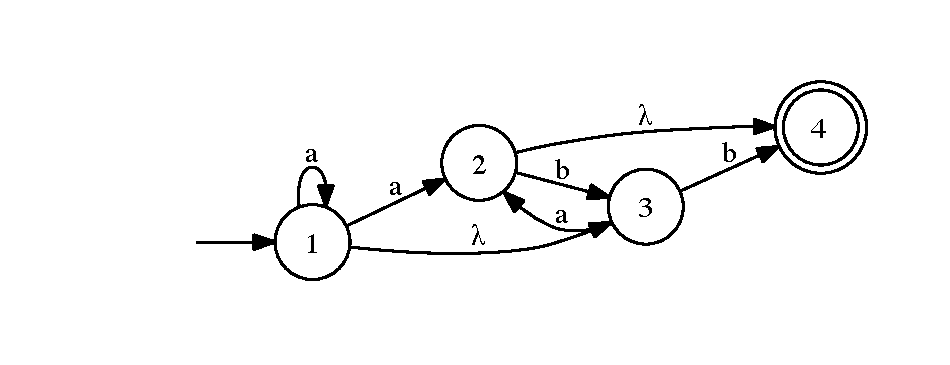
\includegraphics[width=4in]{nfa}
\end{center}
\begin{enumerate}
\item What is the initial state of the DFA using subset construction?\\\\\verb+{1,3}+
\item Draw the equivalent DFA using subset construction.\\\\\\\\\\
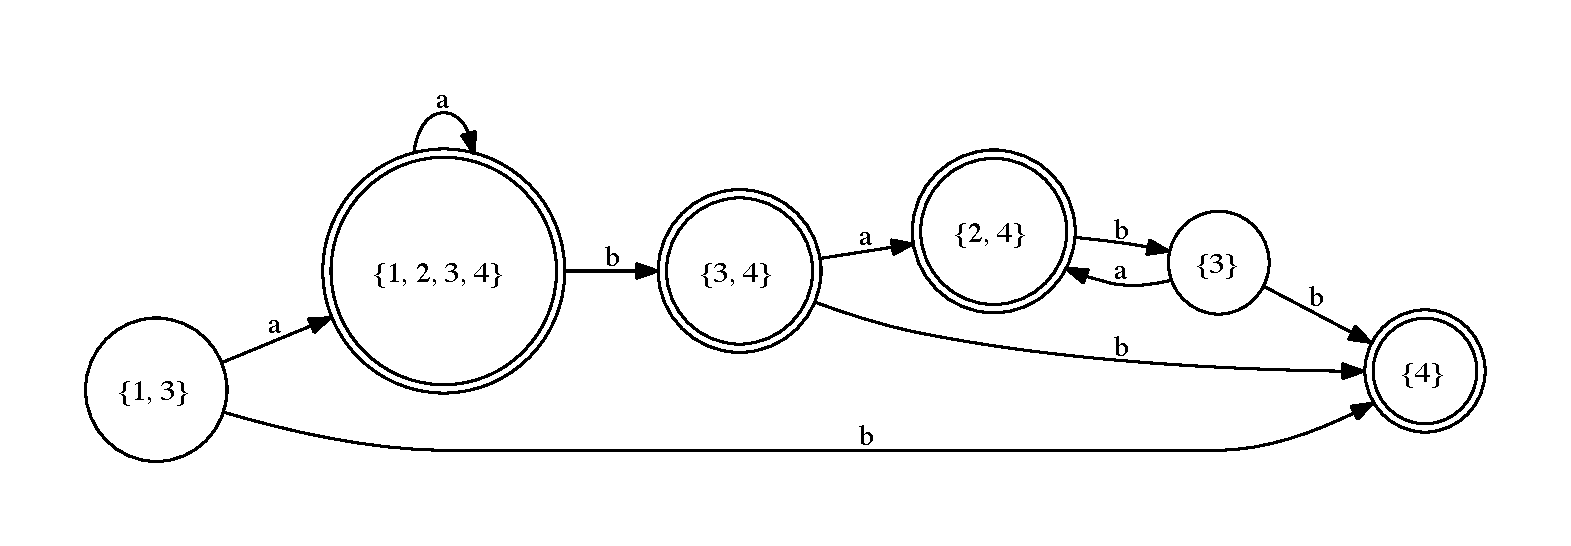
\includegraphics[width=5.4in]{midterm1key-figure}
\item Write the equivalent regular expression.\\\\
$b|aa*(\lambda|b|bb|ba(ba)*(b|\lambda))$
\\\\\\\\\\
\item IPv4 addresses are written as four integers, separated by dots (e.g., \verb+173.203.204.223+). Each integer ranges from 0 to 255. Write a regular expression to match precisely these addresses.\\\\
$(25[0-5]|2[0-4][0-9]|1[0-9]\{1,2\}|[0-9]\char`\\.)\{3\}25[0-5]|2[0-4][0-9]|1[0-9]\{1,2\}|[0-9]$
\end{enumerate}

\section{Context-free languages}
Refer to the context-free grammar below. $S$ is the start symbol. Answer 4 of the following questions. Answer all for extra credit.
\begin{align*}
S &\to T &  T &\to \mathbf{x}\\
S &\to S + T &    T &\to \mathbf{y}\\
S &\to S - T &    T &\to \mathbf{z}\\
S &\to S * T &    T &\to ( S )\\
 S &\to S / T\\
\end{align*}
 \begin{enumerate}
\item Is the grammar above ambiguous? Why or why not?\\\\
\verb+Unambiguous, because the ( symbol forces the parse tree to be formed one way.+\\\\\\
\item Explain why the grammar above is not LL(1).\\\\
\verb+Left recursion, common prefixes.+\\\\\\
\item What is $First(T)$?\\\\
\verb+x, y, z, (+
\\\\\\ 
\item What is $Follow(S)$?\\\\
\verb$+, -, *, /, ), eof$
\\\\\\ % 
\item Perform a leftmost derivation of the following string: $\mathbf{x}*(\mathbf{y}+\mathbf{z})$
\begin{verbatim}
 S => S * T
   => T * T
   => x * T
   => x * (S)
   => x * (S + T)
   => x * (T + T)
   => x * (y + T)
   => x * (y + z)
\end{verbatim}
\end{enumerate}

\section{Extra credit}
Complete any of the following for extra credit.

\begin{enumerate}
\item List all possible $Sentences$ that can be matched by the grammar below.
\begin{align*}
Sentence &\to NounPhrase\ VerbPhrase &     Noun &\to \mathbf{boy}\\
    NounPhrase &\to Article\ Noun    &   Noun &\to \mathbf{ball}\\
    VerbPhrase &\to Verb\ NounPhrase   &  Verb &\to \mathbf{kicked}\\
 Article &\to \mathbf{the}\\ 
\end{align*}
\begin{verbatim}

the boy kicked the ball
the boy kicked the boy
the ball kicked the boy
the ball kicked the ball










\end{verbatim}
\item Rewrite the grammar on the previous page to be LL(1).
\begin{verbatim}
Must eliminate left recursion, common prefixes.

S -> T Y
T -> x
  -> y
  -> z
  -> (S)
Y -> + T
  -> - T
  -> * T
  -> / T
  -> lambda
\end{verbatim}
\end{enumerate}

\end{document}  